\chapter{Графики}
Примеры работы программы при различном начальном состоянии системы, количестве состояний и заполнении матрицы интенсивности приведены на рисунках \ref{g1}--\ref{g4}.

\begin{figure}[h]
	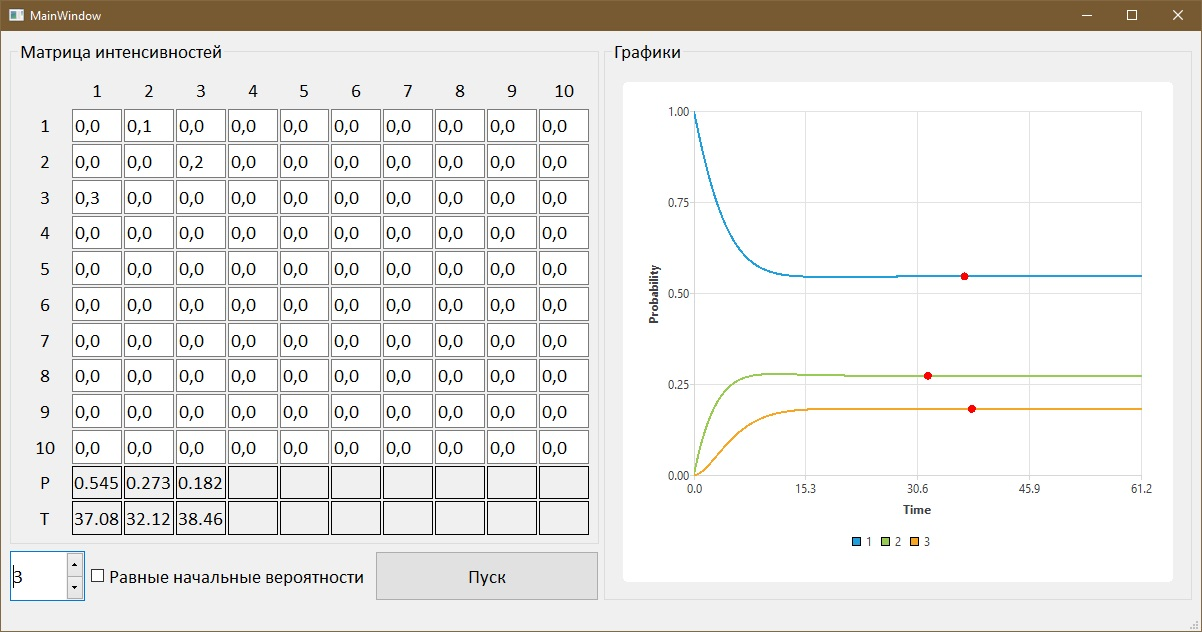
\includegraphics[width=1\linewidth]{inc/img/g1}
	\caption{Графики вероятностей трех состояний}
	\label{g1}
\end{figure}

Проверка результатов (рисунок \ref{g1}):
\begin{equation}
	\left\{\begin{array}{l}
		-0.1 \cdot 0.545 + 0.3\cdot0.182 = 1.0\cdot10^{-4} \\
		-0.2 \cdot 0.273 + 0.1\cdot0.545 = -1.0\cdot10^{-4} \\
		-0.3 \cdot 0.182 + 0.2\cdot0.273 = 0.0
	\end{array}\right.
\label{eq1}
\end{equation}

Вычислим значения вероятностей аналитически:
\begin{equation}
	\left\{\begin{array}{l}
		-0.1 \cdot P_1 + 0.3 \cdot P_3 = 0 \\
		-0.2 \cdot P_2 + 0.1 \cdot P_1 = 0 \\
		-0.3 \cdot P_3 + 0.2 \cdot P_2 = 0 \\
		P_1 + P_2 + P_3 = 1
	\end{array}\right.
	\label{eq2}
\end{equation}

\begin{equation*}
	\left\{\begin{array}{l}
		P_1 = \frac{6}{11} \\
		P_2 = \frac{3}{11} \\
		P_3  = \frac{2}{11}
	\end{array}\right.
\end{equation*}

Значения вычисленные при решении системы уравнений \ref{eq2} совпали с результатами программы \ref{eq1}.

\begin{figure}[h]
	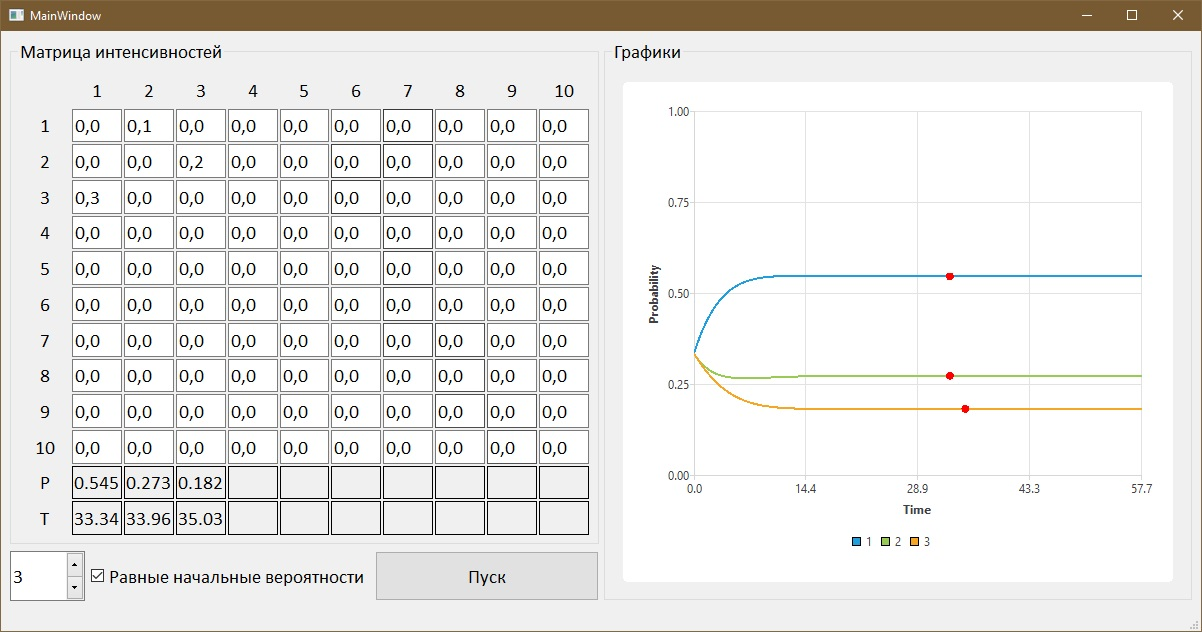
\includegraphics[width=1\linewidth]{inc/img/g2}
	\caption{Графики вероятностей при равных начальных вероятностях}
	\label{g2}
\end{figure}

\newpage
\begin{figure}[h]
	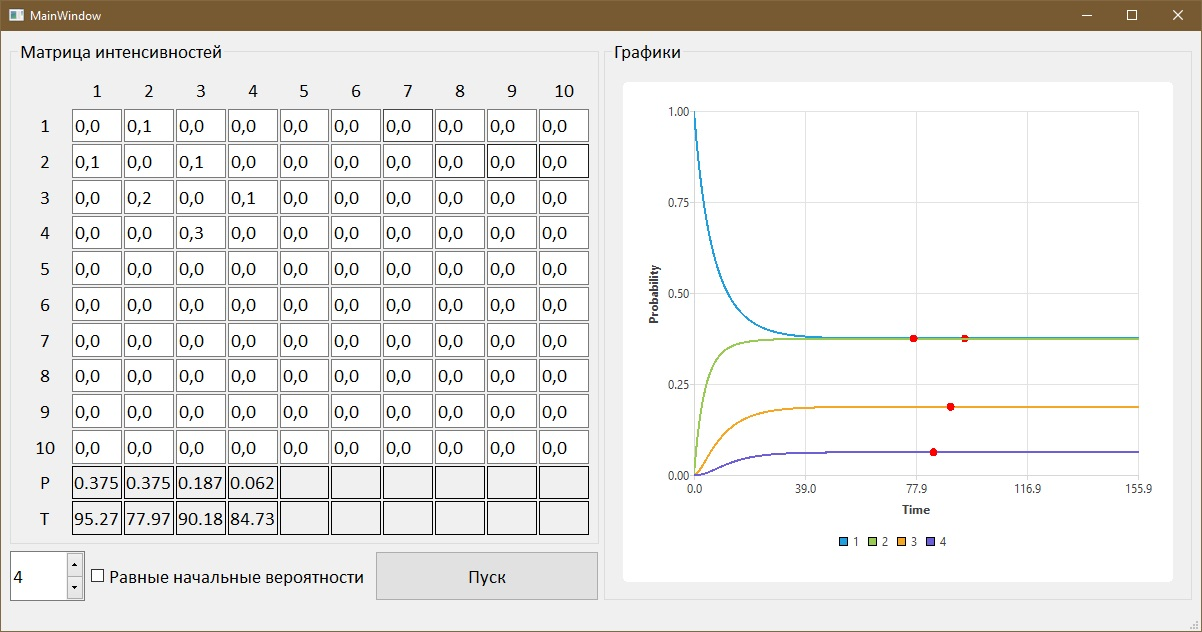
\includegraphics[width=1\linewidth]{inc/img/g3}
	\caption{Графики вероятностей четырех состояний}
	\label{g3}
\end{figure}

Проверка результатов (рисунок \ref{g3}):
\begin{equation}
	\left\{\begin{array}{l}
		-0.1\cdot0.375 + 0.1 \cdot 0.375 = 0.0 \\
		-(0.1+0.1)\cdot0.375 + (0.1\cdot0.375 + 0.2\cdot0.187) = -1.0\cdot10^{-4} \\
		-(0.2+0.1)\cdot0.187 + (0.1\cdot0.375 + 0.3\cdot0.062) = 0.0 \\
		-0.3\cdot0.062 + 0.1\cdot0.187 = 1.0\cdot10^{-4}
	\end{array}\right.
\end{equation}

\newpage
\begin{figure}[h]
	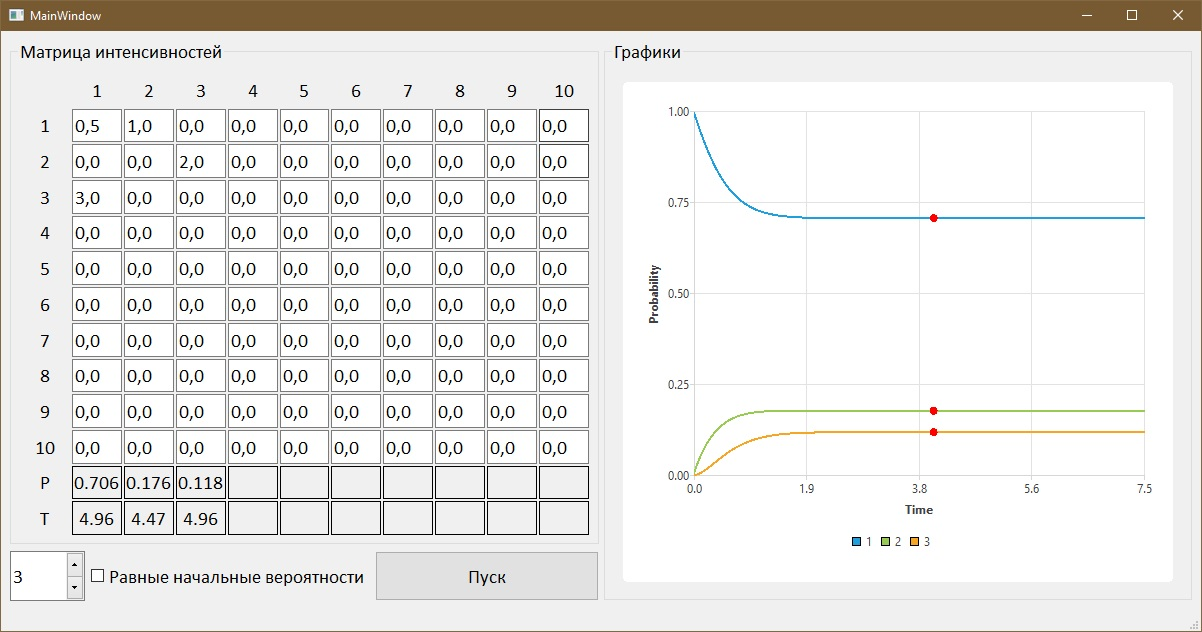
\includegraphics[width=1\linewidth]{inc/img/g4}
	\caption{Графики вероятностей с переходом состояния в само себя}
	\label{g4}
\end{figure}

Проверка результатов (рисунок \ref{g4}):
\begin{equation}
	\left\{\begin{array}{l}
		(-1.0+0.5) \cdot 0.706 + 3.0 \cdot 0.118 = 1.0 \cdot 10^{-3} \\
		-2.0 \cdot 0.176 + (1.0-0.5) \cdot 0.706 = 1.0 \cdot 10^{-3} \\
		-3.0 \cdot 0.118 + 2.0 \cdot 0.176 = -2.0 \cdot 10^{-3}
	\end{array}\right.
	\label{eq1}
\end{equation}